\documentclass[10pt,a4paper]{article}

%================ Packages ================%
\usepackage{polyglossia} % Localisation du document
\usepackage{mathtools} % Ajout d'environnement et + pour les mathématiques
\usepackage{amsfonts} % Ajout de polices pour les équations
\usepackage{amssymb} % Ajout de symboles mathématiques
\usepackage{amsthm} % Permet l'ajout de théorème
\usepackage[load-configurations = abbreviations]{siunitx} % Support unité SI
\usepackage{fontspec} % Changement de police
\usepackage{xcolor} % Coloration de texte
\usepackage{graphicx} % Ajout d'image
\usepackage[margin=2cm, includehead, includefoot, headheight=35pt]{geometry}
\usepackage{fancyhdr} % En-tête et pied de page
\usepackage{subcaption}
\usepackage{listings}
\usepackage[hidelinks]{hyperref}
\usepackage{float}


%================ Configurations ================%
\setdefaultlanguage{french}
\sisetup{locale = FR, detect-all, inter-unit-product ={}.{}, separate-uncertainty = true, multi-part-units=single}

\graphicspath{{./figs/}}
%\setmainfont{Calibri}
%\setmathfont{Cambria Math}
\everymath{\displaystyle}
\newcommand{\titre}{Sherlock 13}
\newcommand{\auteur}{Florian Cormée et Hugo Duarte}

%================ En-tête & Pied et page ================%
\renewcommand{\headrulewidth}{0.05pt}
\lhead{
\includegraphics[height=1cm]{logo_sorbonne.png}}
\chead{\textbf{\titre}}
\rhead{
\includegraphics[height=1cm]{logo_polytech.png}}

\lfoot{\auteur{}}

%================ Nouvelles commandes ================%
\newcommand{\donumber}{\addtocounter{equation}{1}\tag{\theequation}}
\newcommand{\vect}[1]{\ensuremath{\overrightarrow{#1}}}
\newcommand{\dotprod}[2]{(#1 \cdot #2)}
\newcommand{\mat}[1]{\left[ #1 \right]}
\newcommand{\natC}{\ensuremath{\mathbb{N}}}
\newcommand{\relC}{\ensuremath{\mathbb{Z}}}
\newcommand{\realC}{\ensuremath{\mathbb{R}}}
\newcommand{\imgC}{\ensuremath{\mathbb{C}}}
\newcommand{\abs}[1]{\ensuremath{\left| #1 \right|}}
\newcommand{\Ind}{\ensuremath{\mathrm{Ind}}}
\newcommand{\Res}{\ensuremath{\mathrm{Res}}}

 %================ Nouveaux styles de théorèmes ================%
\newtheoremstyle{ex}%name
{3pt}%Space above
{3pt}%Space below
{\color[rgb]{0,0.4,0}}%Body font
{}%Indent amount
{\bfseries}%Theorem head font
{.}%Punctuation after theorem head
{.5em}%Space after theorem head
{}%Theorem head spec(can be left empty, meaning ‘normal’)
\newtheoremstyle{break}%name
{3pt}%Space above
{20pt}%Space below
{}%Body font
{}%Indent amount
{\bfseries}%Theorem head font
{}%Punctuation after theorem head
{\newline}%Space after theorem head
{}%Theorem head spec(can be left empty, meaning ‘normal’)

 %================ Nouveaux théorèmes ================%
\theoremstyle{ex}
\newtheorem*{exemple}{Exemple}
\theoremstyle{break}
\newtheorem{remarque}{Remarque}
\newtheorem{definition}{Définition}
\newtheorem{proposition}{Propostion}
\newtheorem{propriete}{Propriété}
\newtheorem{corollaire}{Corollaire}
\newtheorem{theoreme}{Théorème}

%================ Début du document ================%
\begin{document}
\pagestyle{fancy}
%%%
%% Page de garde
%%%
\thispagestyle{empty}


\includegraphics[height=2cm]{logo_sorbonne.png}
\hfill{}

\includegraphics[height=2cm]{logo_polytech.png}
\vfill{}

\begin{center}
	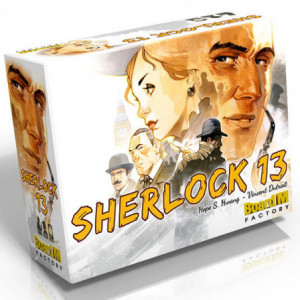
\includegraphics[height=10cm]{sherlock-13.jpg}
\end{center}
\vspace{1cm}

\begin{minipage}[ch]{0.9\textwidth}
	\rule{\linewidth}{0.4pt}
	\vspace{2pt}
	\begin{center}
		\textbf{\LARGE	\MakeUppercase{\titre{}}}
	\end{center}
	\vspace{2pt}
	\rule{\linewidth}{0.4pt}
	\vspace*{1cm}
	\begin{center}
		{\large	\auteur{}}
	\end{center}
\end{minipage}
\vfill{}

\newpage{}


%%%
%% Début du document
%%%
\thispagestyle{empty}
\tableofcontents
\newpage

\setcounter{page}{1}
\section{Diagramme UML de séquence}

\begin{figure}[H]
    \begin{center}
        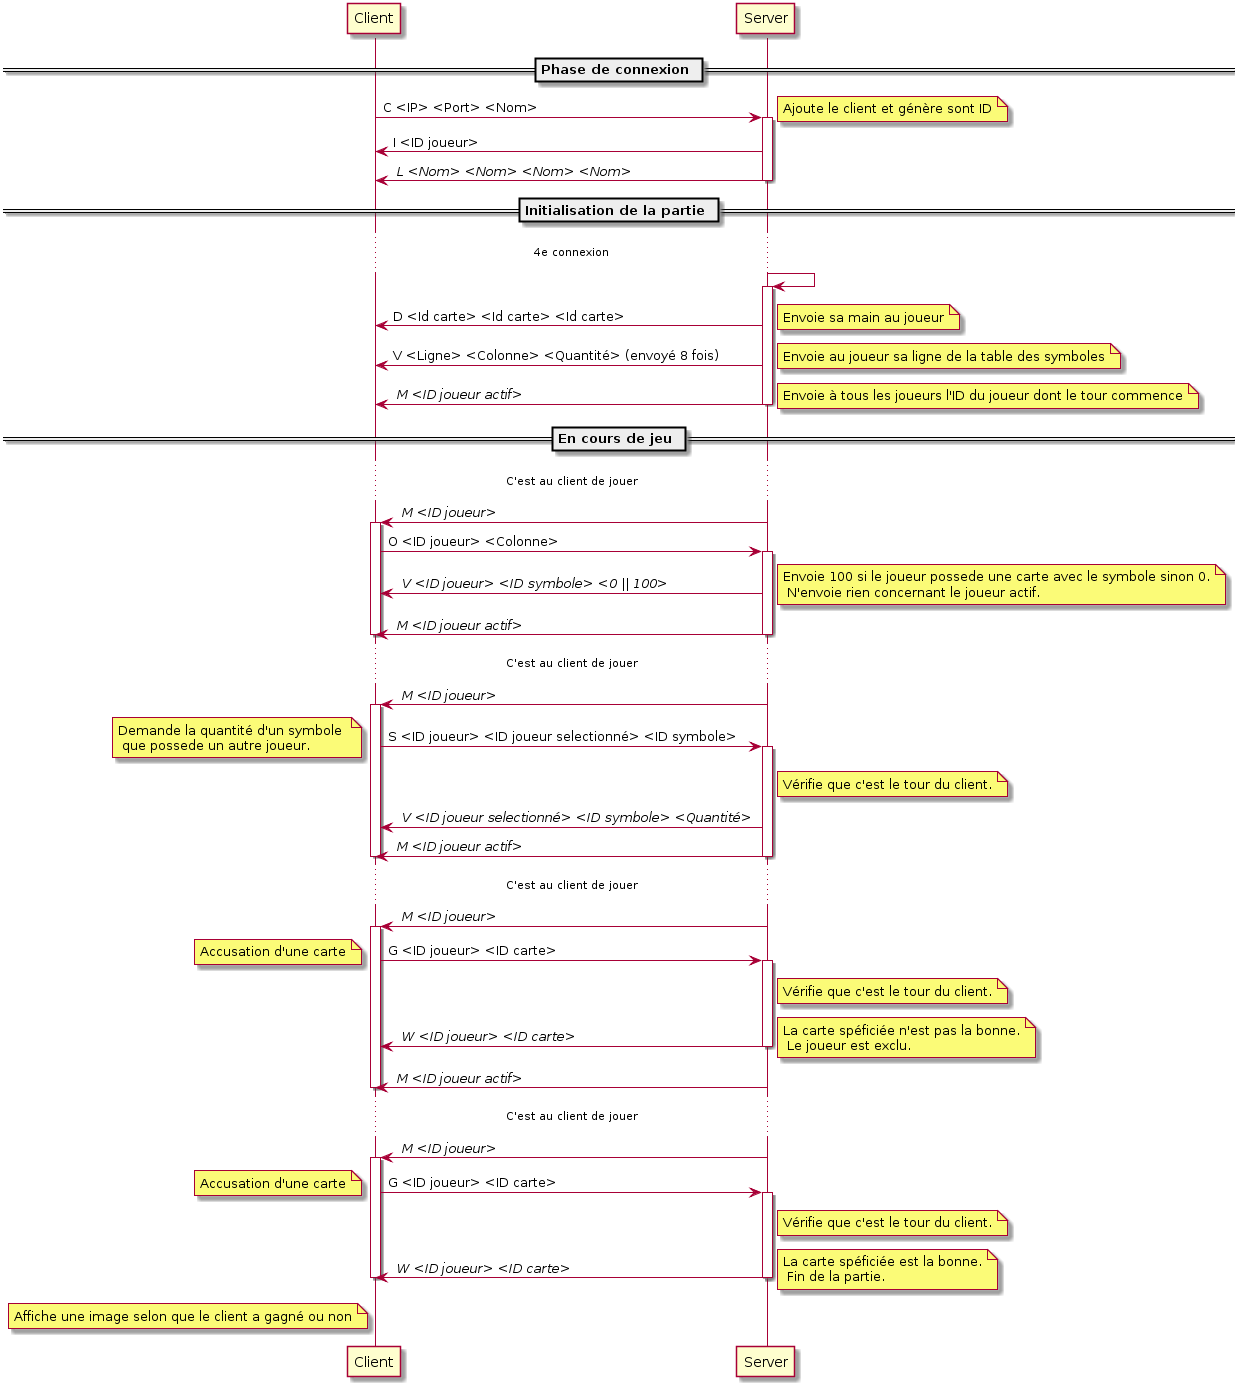
\includegraphics[width=.9\linewidth]{uml_sequence.png}
    \end{center}

    \tiny
    \textit{M <ID joueur actif>}: Commande envoyée à tous les clients connectés.

    <ID joueur>: Argument obligatoire d'une commande.
    \caption{Diagramme UML de séquence}
    \label{fig:uml_sequence}
\end{figure}


\section{Guide utilisateur}

\subsection{Instructions de compilation}

\subsection{Utilisation du client}

\subsubsection{Lancement du client}

Le client sert à générer l'interface graphique à l'utilisateur pour lui permettre de jouer. Pour lancer le client, il faut entrer la commande suivante :
\begin{verbatim}
./sh13.exe <server ip address> <server port> <client ip address> <client port> <player name>
\end{verbatim}
Tous les arguments sont obligatoires. L'adresse ip et le port du serveur doivent être ceux utilisés par le serveur lancé. L'adresse ip du client spécifié peut être localhost. Le port client spécifié doit être disponible. Par exemple, les ports 32 001, 32 002, 32 003, etc. Un nom de joueur doit être renseigné.

\subsubsection{Connection au serveur}

Une fois la commande exécutée, une fenêtre graphique s'ouvrira :
\begin{figure}[H]
    \begin{center}
        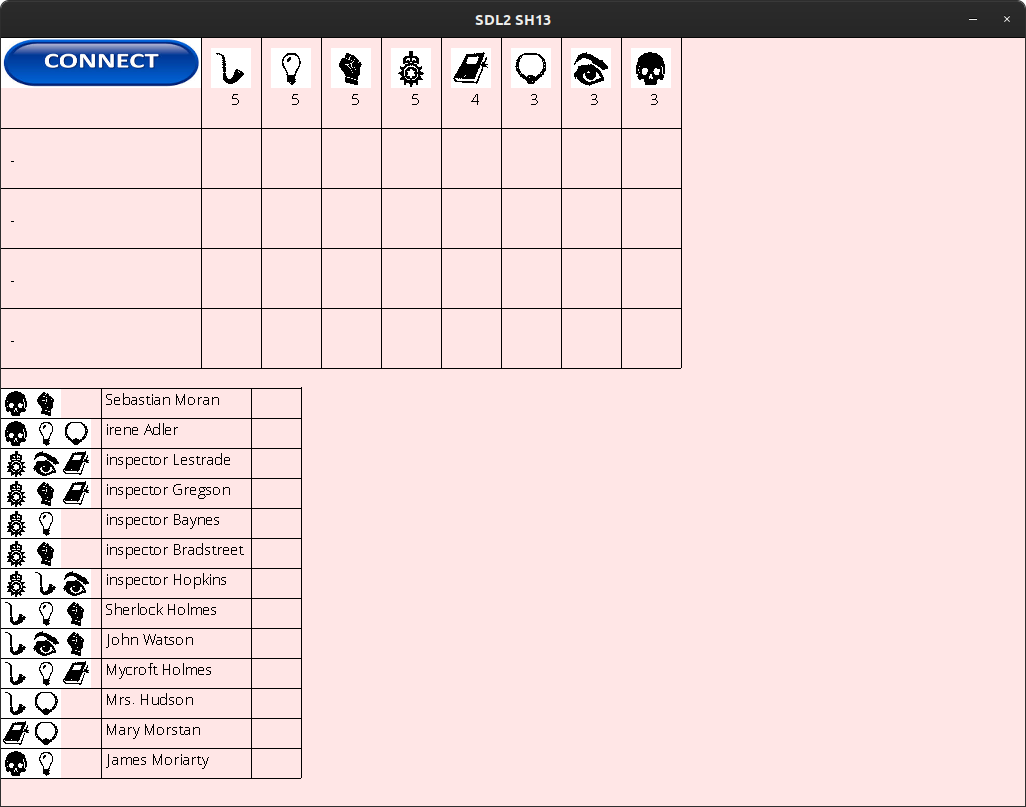
\includegraphics[width=.5\linewidth]{avant_connection.png}
    \end{center}
     \caption{Fenêtre graphique avant connection}
    \label{fig:avant_connection}
\end{figure}
En cliquant sur le bouton connections, vous pourrez avoir accès aux noms des autres joueurs déjà connectés :
\begin{figure}[H]
    \begin{center}
        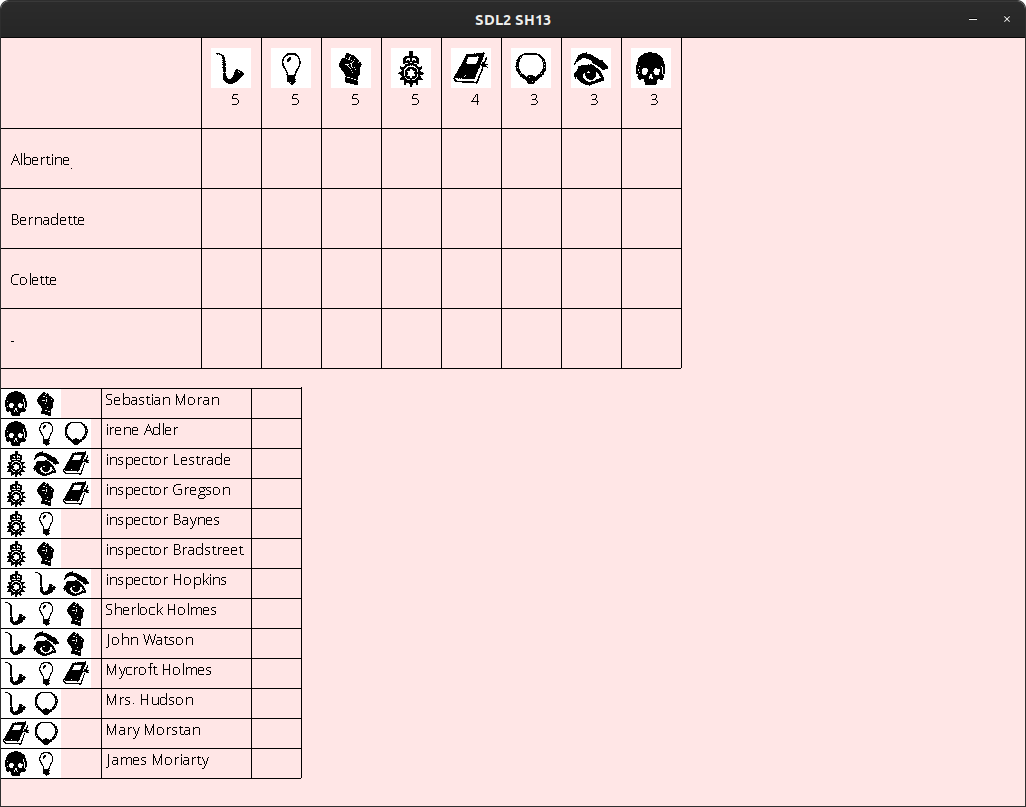
\includegraphics[width=.5\linewidth]{apres_connection.png}
    \end{center}
   	 \caption{Fenêtre graphique après connection}
    \label{fig:après_connection}
\end{figure}
Une fois que le quota de joueurs connectés est atteint, la partie peut commencer !
\begin{figure}[H]
    \begin{center}
        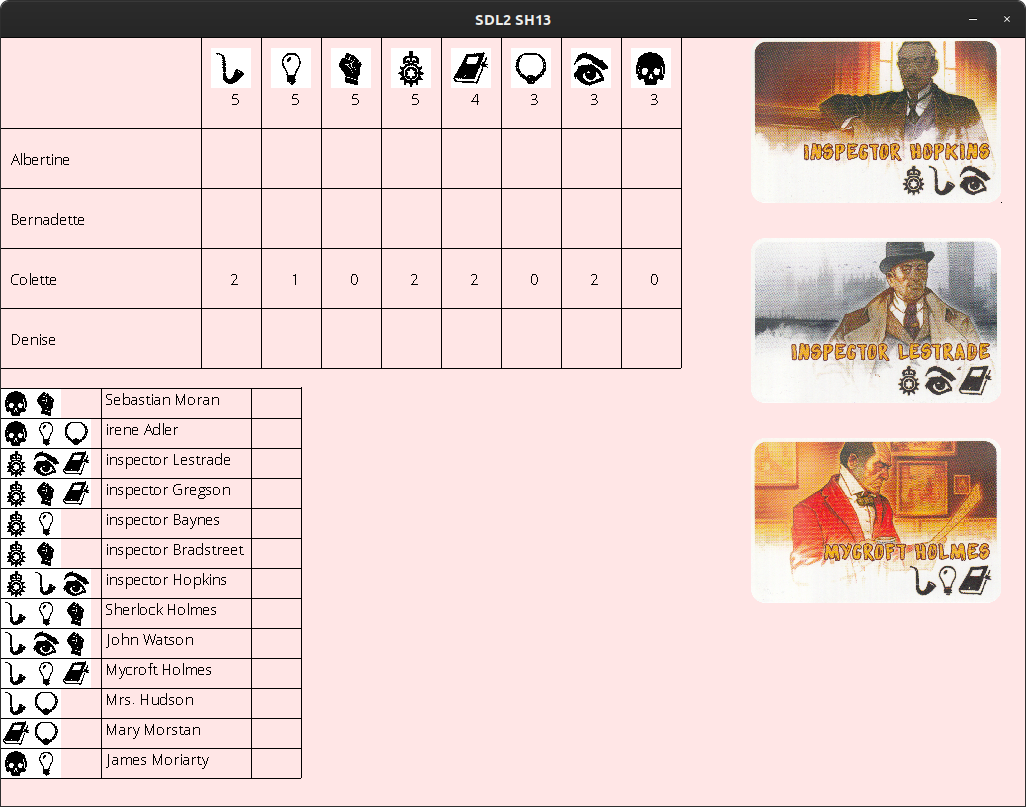
\includegraphics[width=.5\linewidth]{debut.png}
    \end{center}
     \caption{Début de partie}
    \label{fig:debut}
\end{figure}

\subsubsection{Actions disponibles}

Une fois sur la partie lancée, plusieurs actions sont disponibles :
\begin{description}
  \item[Utilisation du mémo] : (figure \ref{fig:memo}) En cliquant dans les cases à côté des noms des différents personnages, vous pouvez indiquer qui vous sembles présent dans les mains des différents joueurs.
  \item[Savoir qui possède un symbole] : (figure \ref{fig:qui_symbole}) En cliquant sur la case du symbole en question et en confirmant son action (en cliquant sur le bouton go), vous pourrez savoir quels joueurs possèdent des personnages liés à ce symbole.
  \item[Savoir combien de fois un joueur possède un symbole] : (figure \ref{fig:combien_symbole}) En cliquant sur la case du symbole en question ainsi que la case du joueur souhaité et enfin en confirmant son action (en cliquant sur le bouton go), vous pourrez savoir combien de personnage sont liés à ce symbole dans la main de l'autre joueur.
  \item[Accuser un des personnages] : (figure \ref{fig:accusation}) En cliquant sur le nom d'un personage et en confirmant son action (en cliquant sur le bouton go), vous lancez une accusation.
\end{description}

\begin{figure}[H]
     \centering
     \begin{subfigure}{.45\linewidth}
       \centering
           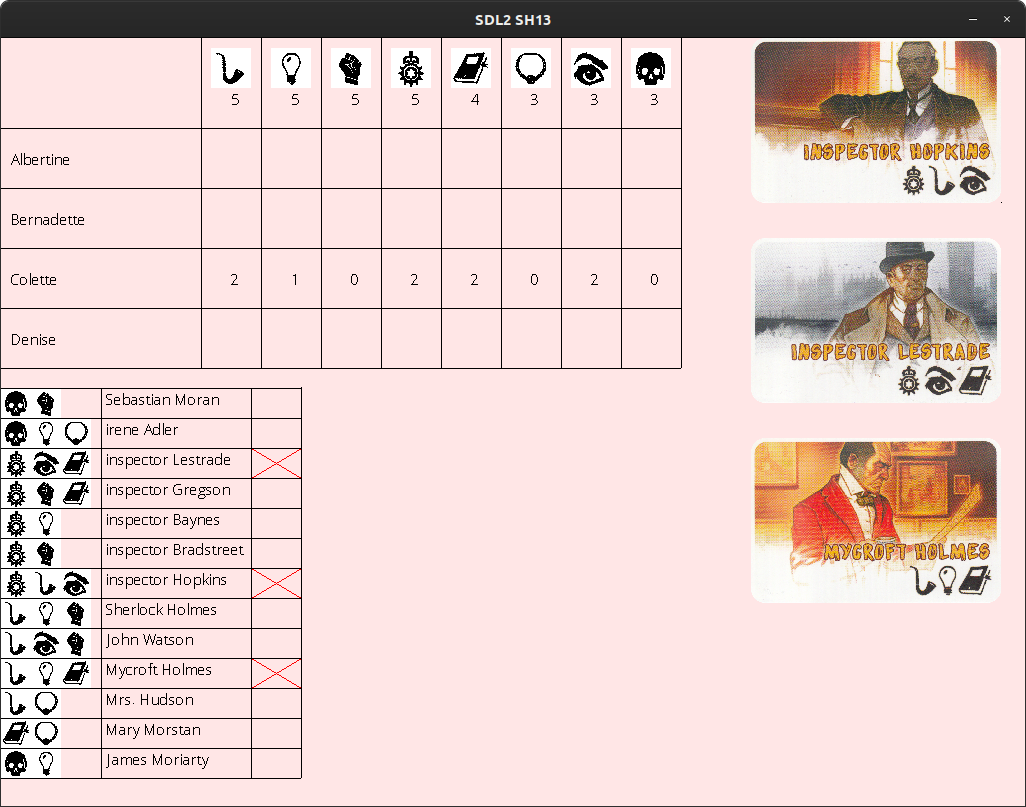
\includegraphics[width=\linewidth]{memo.png}
       \caption{Utilisation du mémo}
       \label{fig:memo}
     \end{subfigure}
     \hspace{1em}
     \begin{subfigure}{.45\linewidth}
	  \centering
       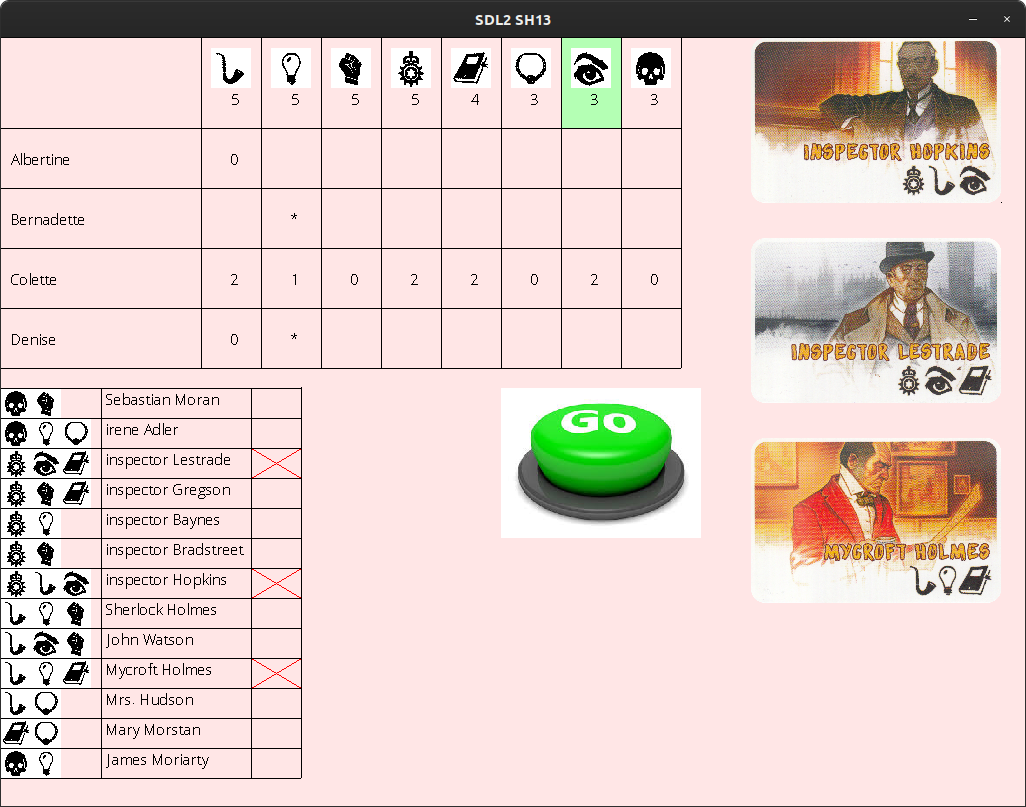
\includegraphics[width=\linewidth]{qui_symbole.png}
       \caption{Savoir qui possède un symbole}
       \label{fig:qui_symbole}
     \end{subfigure}
     \hspace{1em}
     \begin{subfigure}{.45\linewidth}
         \centering
         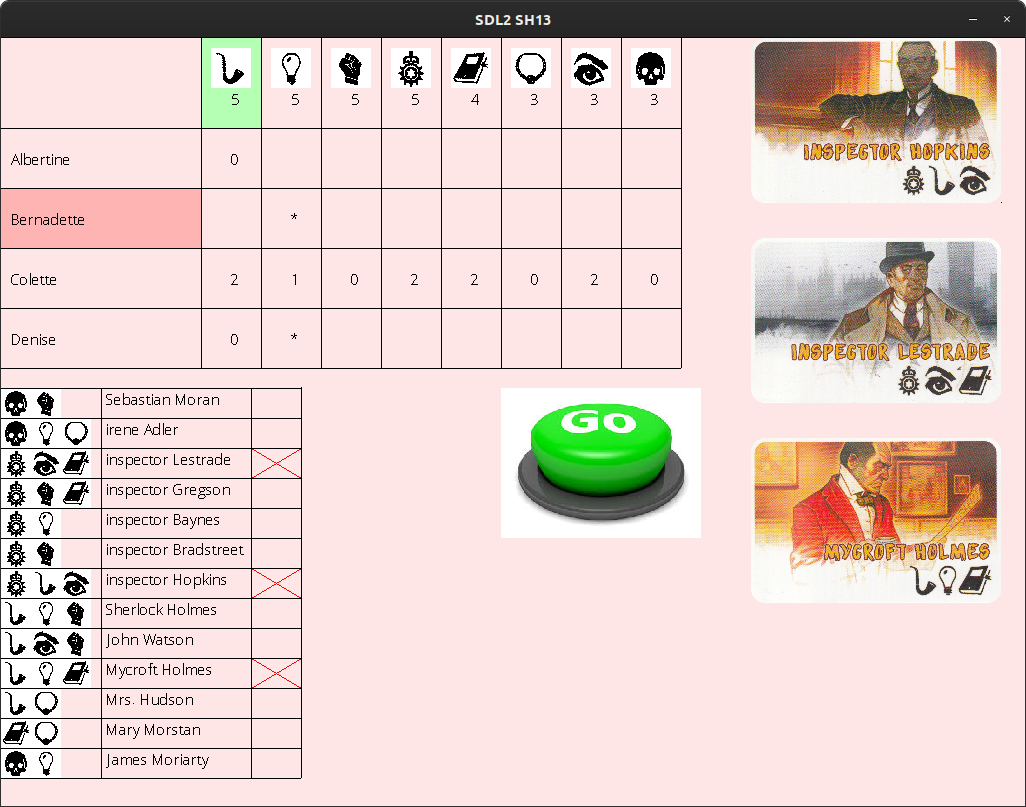
\includegraphics[width=\linewidth]{combien_symbole.png}
        \caption{Savoir combien de fois un joueur possède un symbole}
       \label{fig:combien_symbole}
     \end{subfigure}
     \hspace{1em}
     \begin{subfigure}{.45\linewidth}
	 \centering
           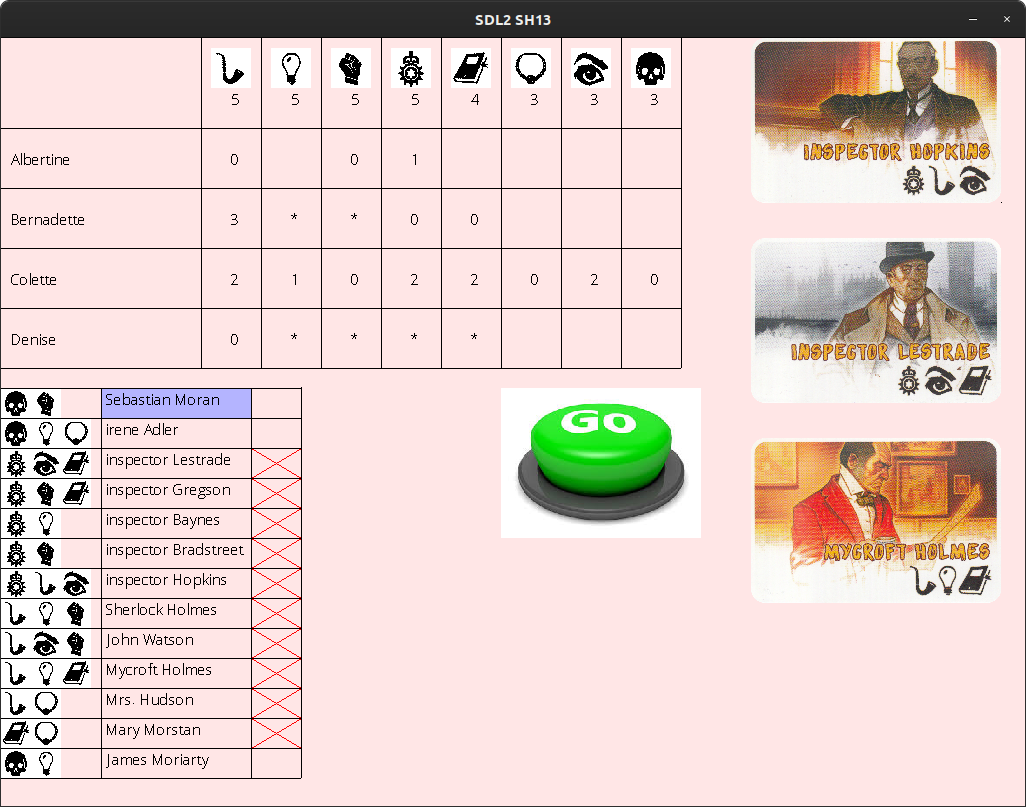
\includegraphics[width=\linewidth]{accusation.png}
      	   \caption{Accuser un des personnages}
       \label{fig:accusation}
     \end{subfigure}
     \caption{Captures des différentes actions} 
\end{figure}

Pour ces trois dernières actions, il est nécessaire de cliquer sur le bouton go (et donc mettre fin à son tour) pour les valider. Pour annuler la sélection, il suffit de cliquer en dehors de tout encart.

Enfin, une fausse accusation entraîne la défaite du joueur tandis que la bonne accusation apporte sa victoire.

\begin{figure}[H]
     \centering
     \begin{subfigure}{.45\linewidth}
         \centering
         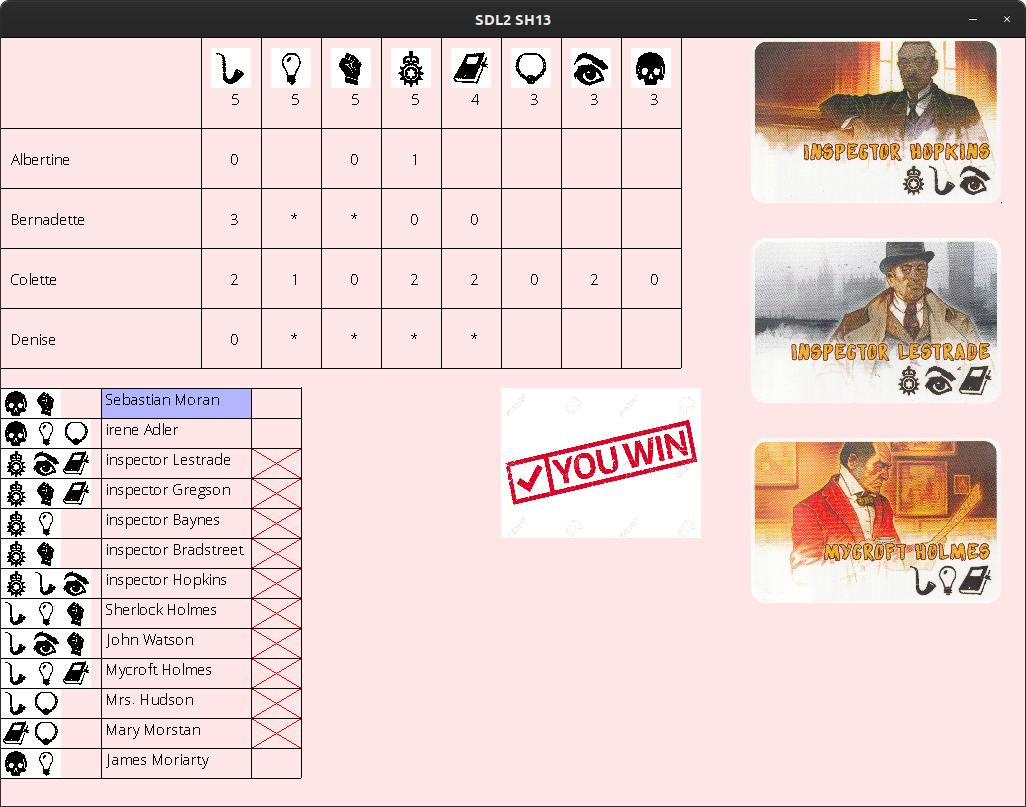
\includegraphics[width=\linewidth]{perdre.png}
         \caption{Victoire}
		\label{fig:victoire}
     \end{subfigure}
     \hspace{1em}
     \begin{subfigure}{.45\linewidth}
         \centering
         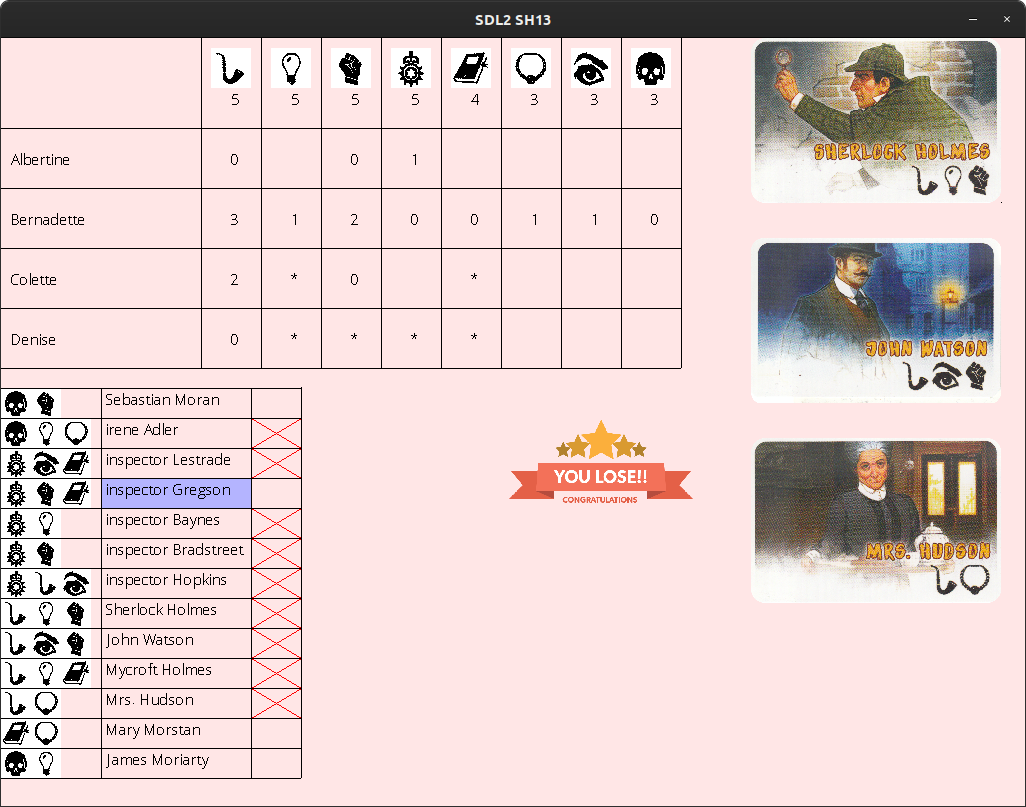
\includegraphics[width=\linewidth]{gagner.png}
         \caption{Défaite}
		\label{fig:defaite}
     \end{subfigure}
\end{figure}

\subsubsection{Fermeture du client}

Pour mettre fin au programme, il suffit de cliquer sur la croix de fermeture de la fenêtre graphique ou de sélectionner sa console et appuyer sur les touches \verb|Ctrl + C|.

\subsection{Utilisation du serveur}

En tant qu'utilisateur, les intéractions avec le serveur, se limite à l'exécuter
et à l'arrêter. Pour lancer le serveur, il suffit d'entrer la commande suivante:
\begin{verbatim}
    ./server <port>
\end{verbatim}
Le port est un argument obligatoire. Le port spécifié doit être disponible. Par exemple, le port 32000.

Afin de ne pas interrompre le chat en fin de partie, le serveur ne s'arrête pas. Pour l'arrêter, sélectionnez sa console et appuyez sur les touches \verb|Ctrl + C|.



\section{Fonctionnement général du code}

Cette section n'a pas pour ambition d'expliquer en détail le fonctionnement du
code du client et du serveur. Néanmoins, elle présente le principe de
fonctionnement et l'agencement du code qui a été remanier pour rendre le code
plus lisible.

\subsection{Fonctionnement du client}

\subsubsection{Présentation de l'algorithme}

Au lancement, le client initialise ses variables, se connecte au serveur et
génère l'interface graphique. On rentre ensuite dans la boucle principale qui
est découpé en trois partie. Dans un premier temps, le programme analyse les
interactions que l'utilisateur a avec la fenêtre graphique et envoie les
commandes associées au serveur. Ensuite, si une requête est reçu du serveur, il
exécute les commandes associées. Enfin, il met à jour la fenêtre graphique à
l'aide des nouvelles informations reçu. La boucle est quittée quand la fenêtre
est fermée et les différents objets graphiques sont détruits.

\subsubsection{Répartition du code}

Afin de rendre le code source du client plus lisible, nous l'avons découpé en
de multiples fichiers et fonctions. Ce découpage est thématique. Nous avons
aussi essayé de ne pas avoir des fonctions de plus de 100 lignes ainsi que des
fichiers de moins de 500 lignes de code.

Ainsi, les fichiers \verb=cartes.h= et \verb=cartes.c= regroupent les fonctions
et les variables globales liées aux cartes.

La communication a été abstraite avec les fichiers \verb=com.h= et \verb=com.c=.
Ces fichiers proposent des fonctions d'envoi de message au serveur.

Les fichiers \verb=gui.h= et \verb=gui.c= gèrent les fonctions liées à
l'interface graphique ainsi que toutes les variables liées à l'environnement
graphique. De cette façon, \verb=sh13.c= ne contient que la boucle principale.


\subsection{Fonctionnement du serveur}

\subsubsection{Présentation de l'algorithme}

Tout d'abord, le serveur initialise ses variables. Les adresses des clients sont
\verb|localhost| et le port est initialisé à une valeur impossible. Le serveur
mélange les cartes et rempli sa table de vérité. sors et le programme
comptabilise la quantité de chaque symbole que possédera chacun des joueurs.

Suite à cela, le programme prépare un socket en tant que serveur lié au port
passé en argument. Dès lors, le programme attend la réception d'un message.

À la réception d'un message le programme acceptera différentes commandes selon
son état. Comme le montre la figure \ref{fig:uml_sequence}, à l'état initiale,
le serveur n'accepte que des demandes de connection. Une fois les quatres
connections établies, le serveur envoie ses cartes et sa ligne de la table de
vérité à chaque joueur. Puis il annonce le début du tour du premier joueur.
Enfin, le programme change d'état pour gérer les commandes liées au déroulement
du jeu.

Dans ce second état, le serveur accepte les commandes d'accusation et de
questionnement. Quand l'une d'elles est réceptionnée, le programme vérifie que
l'expéditeur est bien le joueur actif, dans le cas contraire, un message est
affiché dans la console et la requête est refusée. Une fois la requête
accomplie, le serveur annonce l'identifiant du joueur suivant. L'opération se
répète jusqu'à se qu'un jour parvienne à démasquer le coupable ou que tous les
joueurs ont été éliminé, ceci se produit lorsqu'une fausse accusation est
lancée.

\subsubsection{Répartition du code}

Afin de rendre le code source du serveur plus lisible, nous l'avons découpé en
de multiples fichiers et fonctions. Se découpage est thématique. Nous avons
aussi essayé de ne pas avoir des fonctions de plus de 100 lignes ainsi que des
fichiers de moins de 500 lignes de code.

Ainsi, les fichiers \verb=cartes.h= et \verb=cartes.c= regroupes les fonctions
et les variables globales liées aux cartes.

La communication a été abstraite avec les fichiers \verb=com.h= et \verb=com.c=.
Ces fichiers proposent des fonctions d'envoie de message à un client ou à tous
les clients. Ils regroupent aussi les variables globales contenant les adresses
des clients.

Les fichiers \verb=msg.h= et \verb=msg.c= ajoute de l'abstraction vis-à-vis du
formatage d'un message. De cette façon, \verb=server.c= ne contient que la
boucle principale.


\end{document}
